\documentclass[]{report}

\usepackage{graphicx}
\usepackage{bookmark}

% Title Page
\title{Technical Manuel \newline Yavin IV Defence System}
\author{Team Dirac}


\begin{document}
\maketitle

\chapter{Introduction}
\section{Document Identification}
This document describes the design of the Yavin IV Defence System. This document is prepared by Group DIRAC for assessment in MTRX3700 in 2014.

\section{System Overview}
<A brief statement of the purpose of the system or subsystem to which this document applies>
The Yavin IV Defence System is designed to provide accurate, low cost tracking for Death Stars and other similar objects.

\section{Document Overview}
<A short "road map" of the document, to provide an orientation for the reader. Summarise the purpose and contents of this document.>
This document describes the detailed technical specifications and functionality for the entire system. This includes the entire system design, implementation and usage.

\section{Reference Documents}
The present document is prepared on the basis of the following reference documents, and should be read in conjunction with them.
	<Insert relevant documents>
\subsection{Acronyms and Abbreviations}


\begin{center}
	\begin{tabular}{| l | c |}
		\hline
		Acronym & Meaning \\ \hline \hline
		Thing & Meaning of Thing \\ \hline
		Stuff & Meaning of Stuff \\
		\hline
	\end{tabular}
\end{center}

\chapter{System Description}
This section is intended to give a general overview of the basis for the Yavin IV Defence System system design, of its division into hardware and software modules, and of its development and implementation.

\section{Introduction}
The system is broken into 
<Give a technical description of the function of the whole system, in terms of its constituent parts, here termed modules. Generally, a module will have hardware and software parts.

\section{Operational Scenarios}
<Describe how the system is to be used. There may be several different ways that it ca be used perhaps involving different users, or classes of user. Present case diagrams here if you are using them. Each operational scenario is a part through a use case diagram - a way of using the system, with different outcomes or methods of use. You should also consider the various failures that may occur, and the consequences of these failures. >

\section{System Requirements}
The operational scenarios considered place certain requirements on the whole Yavin IV Defence system, and on the modules that comprise it.
<Statement of requirements that affect the system as a whole, and are not restricted to only a subset of its modules.>

\section{Module Design}
<Describe the breakdown of the design into functional modules. Each module probably contains both software and hardware.
Then include a section like the following 2.5 for each module. Not all of the sub-headings may be relevant for each module.>

The system was broken down into a number of independent modules which contain their own private variables, functions etc. Fig. \ref{fig:Modules} gives an approximate diagrammatic representation of the way the modules fit together.

\begin{figure}
\centering
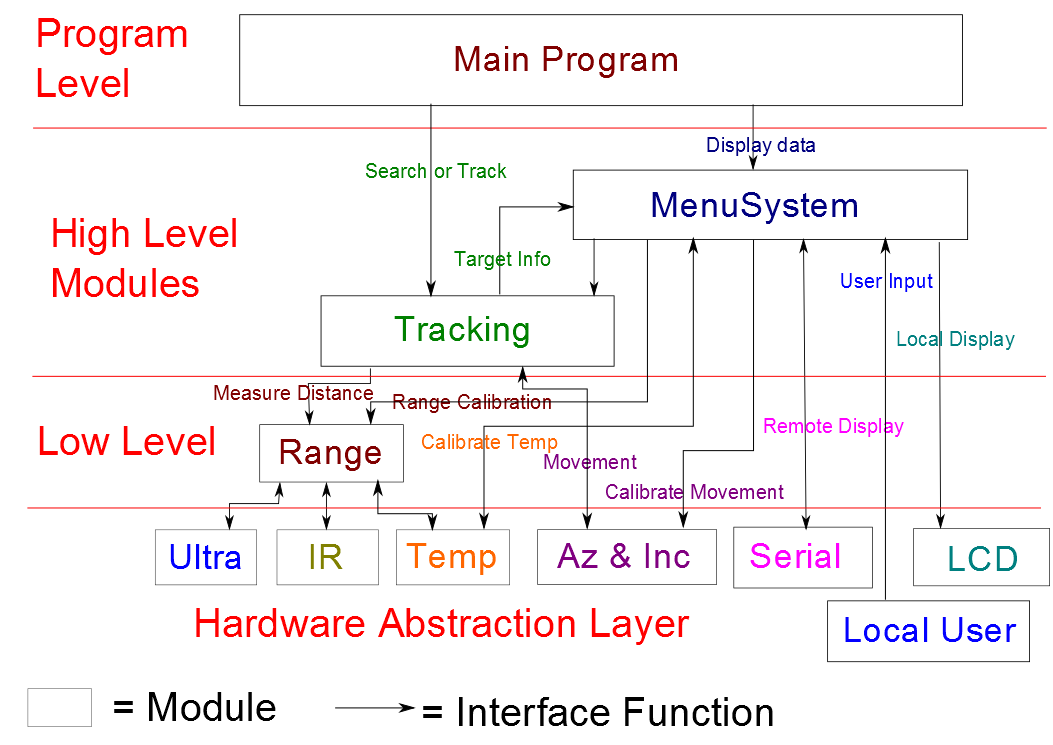
\includegraphics[width=0.7\linewidth]{../Diagrams/Modules}
\caption[Modules]{Conceptual Diagram of the module breakdown and interaction between modules.}
\label{fig:Modules}
\end{figure}



\section{Serial}
\subsection{Description}
The serial module takes care of all communication (transmit and receive) over the serial UART (rs-232) port.

\subsection{Functional Requirements}
\subsubsection{Inputs}
The only external input to the system is characters or strings to transmit. \newline 
Either transmit, or transmitROM must be used depending on if the string is in RAM or ROM. The incorrect usage will result in printing nothing. \newline
Sending a string which in not null terminated will result in unexpected behaviour, most probably filling and overflowing the buffer until a null is reached. \newline
Sending a different datatype such as a float instead of a char will result in syntax errors, but other integer types may be casted into a char, truncating data and resulting in unexpected results. Again, the function only takes char's and integers must first be converted to a char array.

\subsubsection{Processes}
The following processes must be operational:
\begin{itemize}
	\item The circular buffer functionality - pushing and popping characters from buffers must work properly for the module to operate.
\end{itemize}


\subsubsection{Outputs}
The system must output the following to work correctly: 
\begin{itemize}
	\item exact characters received over the serial line in the correct order.
\end{itemize}

\subsubsection{Timing}
The serial module must be capable of:
\begin{itemize}
	\item Storing characters as soon as they are received over serial
	\item Retaining received characters until they are handled
	\item Retaining transmission characters until they can be transmitted
\end{itemize}

\subsubsection{Implemented Basic Functionality}
The serial module implements the following basic functionality:
\begin{itemize}
	\item Functioning receive and transmit serial interrupts
	\item Configure function to set up the module
	\item Separate circular buffers to store data received and data to be transmitted
	\item Public Function to add data to the transmission buffer
	\item Public Function to read from received buffer, and check if anything has been received
\end{itemize}

\subsection{Non-Functional Requirements}
\subsubsection{Performance}
The serial module should have the following performance characteristics:
\begin{itemize}
	\item Very fast ISR's - to affect background code, and other waiting interrupts as little as possible
	\item Very low ISR latency - So no characters are missed, and the the module transmits almost as soon as possible.
\end{itemize}

\subsubsection{Interfaces}
The following interface requirements are desirable:
\begin{itemize}
	\item Complete isolation/modularisation (e.g. no global interrupts) - the buffers are not accessible to the rest of the program
	\item Very simple, intuitive interface functions taking 1 or no arguments that are appropriately named.
	\item As simple operation as possible - E.g. configureSerial() then transmit().
\end{itemize}

\subsubsection{Design Constraints}
The design of the serial module was constrained by the following:
\begin{itemize}
	\item Only High and Low ISR's on the PIC - Needed a public ISR function that is called when a serial interrupt is fired - Reduced modularity and interrupt response
	\item Very little memory on the PIC - buffers were restricted to 30 characters
\end{itemize}

\subsubsection{Implemented Additional Functionality}
In addition to the required functionality above, the serial module also offers the following functionality:
\begin{itemize}
	\item Push Null terminated strings to the transmit buffer
	\item Check if carriage return, or esc has been received
	\item Pop an entire string from the receive buffer up to a carriage return
	\item Clear the buffers
	\item Receiving backspace characters removes the last characters from the buffer (if not CR or ESC)
	\item Read a string form program memory and transmit
	\item Peek - Read character without removing from buffer
	\item Indicate if transmit buffer is empty (all messages sent)
\end{itemize}

\subsection{Conceptual Design:}
The serial module is INTERRUPT DRIVEN. This means that any background code can be running while the module is transmitting and/or receiving data over the serial line, and no serial data should ever be missed, overlooked or cut out. \newline
The module contains two circular buffers: a transmit buffer and a receive buffer. These buffers are NOT accessible by the rest of the program. Rather, the module provides a public function transmit() which takes a string, and places it into the transmit buffer. Anything in this buffer is then transmitted character by character when the transmit ready interrupt fires. \newline
Whenever a character is received over serial it is stored in the received buffer by an interrupt. Again this buffer is NOT accessible to the rest of the program. Rather it provides a number of functions to interact with it. The most commonly used of which is the readString() function, which returns everything in the buffer up to a carriage return (e.g. a line of input entered by the user). \newline
This serial module also allows users the opportunity to remove or change data they have already transmitted. If a backspace is received, then instead of storing it in the receive buffer it will remove the last received character from the buffer if that character is not a Carriage Return, Newline, or Escape operator. This enables a much more more user friendly system as otherwise there would be no way to fix any syntax error without pressing enter, getting an error and starting again. Furthermore, without this feature, if a user did backspace and change an input it would result in completely unexpected behaviour. \newline
Fig. \ref{fig:SerialModule} shows a conceptual diagram of the function of the serial module.

\begin{figure}
	\centering
	\includegraphics[width=0.7\linewidth]{"../Diagrams/Serial Module"}
	\caption[Serial Module]{Shows Conceptual Diagram of Serial Module -> Received input stored by interrupts into circular buffer to await pop commands. Transmit data pushed onto buffer which is transmitted via interrupts}
	\label{fig:SerialModule}
\end{figure}

\subsubsection{Assumptions Made}
The module assumes that the buffers will never be overfilled, i.e. is able to transmit data faster than being written into buffer, or that input is being handled in a timely fashion. Failing this, it is assumed that the oldest data (which is overwritten) is the least meaningful, and that loosing some data will not create catastrophic error in the system. It is recommended to include a wait if sending large blocks of text over serial.

\subsubsection{Constraints on Serial Performance}
The main constraints on the serial module performance are:
\begin{itemize}
	\item Baud Rate
	\item Interrupt Latency
\end{itemize}
The baud rate sets a maximum rate data can be transferred, which along with the buffer length restricts the rate at which data can be written to the transmit buffer without an overflow occurring.
The interrupt latency is the time delay between the interrupt firing and the actual event. This is generally very small (we found ~300$\mu$s), but a high latency could miss characters being received.

\subsection{Interface}
Refer to the Technical User Manual For detailed explanations of the interface functions and how to use them.

\section{Pan Tilt}
\subsubsection{Description}
The Pan Tilt module is responsible for interfacing and driving the pan tilt mechanism. This primarily consists of generating the PDM signals required to send dictate the position of the servo's.

\subsection{Functional Requirements}
\subsubsection{Inputs}
The module takes the following inputs
\begin{itemize}
	\item The Direction as a direction struct
\end{itemize}

\subsubsection{Processes}
The following processes must be operational for the functionality of the module
\begin{itemize}
	\item 
\end{itemize}

\subsubsection{Outputs}
The only program output is the current pan tilt direction. \newline
The only other output is the PDM outputs to the servo which dictate their position.

\subsubsection{Timing}
The Pan Tilt module must have very precise timing to ensure that the servo positions are maintained precisely.
\begin{itemize}
	\item Module must be interrupt driven
	\item Must have very low interrupt latency
	\item PDM's must be offset so that the interrupts for elevation and azimuth don't interfere and block each other
	\item Delay after movement function to allow the servo's to move to that position
\end{itemize}

\subsubsection{Failure Modes}
The Pan Tilt module includes the following assurances against failure:
\begin{itemize}
	\item New delay information is only set at the end of a cycle to guarantee the PDM frequency
	\item Validation function to ensure that the high time to within the specified range in the datasheet  
\end{itemize}

\subsubsection{Implemented Basic Functionality}
The Pan Tilt module includes the following basic functionality:
\begin{itemize}
	\item Configure function to set up the module
	\item Move function to move to any valid position
	\item Get Direction function to return the current direction
\end{itemize}

\subsection{Non-Functional Requirements}
\subsubsection{Performance}
The module should have the following performance characteristics to perform well:
\begin{itemize}
	\item Very low interrupt latency
	\item Adjustment for interrupt latency
\end{itemize}

\subsubsection{Interfaces}
The following interface characteristics are desirable:
\begin{itemize}
	\item Complete Isolation/modularity so that the rest of the program does not have access to any of the functionality of the module, but merely sets the direction of the Pan-Tilt module
	\item Very simple, intuitive interface functions taking 1 or no arguments that are appropriately named.
	\item Very simple module operation, such as configuration and move to desired location
\end{itemize}

\subsubsection{Implemented Additional Functionality}
The following additional functionality has been implemented for the Pan Tilt Module
\begin{itemize}
	\item Incremental move function
	\item Increment fine function for greater precision
	\item Updated function to indicate whether a new delay setting has actually been written into the system yet
\end{itemize}

\subsection{Conceptual Design}
This module uses a single output compare module to create the delays necessary to generate the PDM's of the desired duty cycle. Due to the interrupt latency of approximately 300$\mu$s, the PDM's are staggered so that the interrupt calls will never be closer than approximately 0.04 seconds. The full available duty cycle (1000$\mu$s) is divided over the given angular range. There is also an angular offset for calibration reasons. The Delay object is then created to define the necessary delays to create the desired PDM.
NOTE: This module is interrupt driven, so the Interrupt.c file must be included in the project for it to work. \newline
A data Flow diagram of the Pan Tilt Module is shown in Fig. \ref{PanTiltPins}.

\begin{figure}
\centering
\includegraphics[width=0.7\linewidth]{"../Diagrams/Pan Tilt Data Flow Diagram"}
\caption[Pan Tilt Dataflow Diagram]{Dataflow diagram showing the transition from inputted direction to servo direction}
\label{fig:PanTiltDataFlowDiagram}
\end{figure}

\subsubsection{Assumptions Made}
The largest assumption made is that the clock frequencies in the code match those of the actual clock. Common.h defines the clock frequencies of the PICDEM and Minimal Boards which can be switched between. But there is no way for the system to verify the frequency of the clock, and if the clock is not the same then the PDM frequency will not be 50Hz, which can damage the servo's if faster. \newline
The module does not assume that the interrupts fire instantly after the timing event, but that there is an approximately constant latency time, which is found experimentally, included as a \# define, and tuned.

\subsubsection{Constraints on Pan Tilt Performance}
The Pan Tilt module is restricted to the servo range of motion. Also the actual position is entirely dependant on the calibration as they merely take a PDM input.

\subsubsection{Interface}
Refer to the Technical User Manual For detailed explanations of the interface functions and how to use them.

\section{Range}
\subsection{Description}
The range module uses the IR, Ultrasonic and temperature sensors to take range measurements.

\subsection{Functional Requirements}
\subsubsection{Inputs}
The range module takes no real inputs

\subsubsection{Processes}
The range module requires the following processes to function properly
\begin{itemize}
	\item Sample the Ultrasonic and IR sensors
	\item Convert the sensor output to a range
	\item Fuse the ranges from different sensors 
\end{itemize}

\subsubsection{Outputs}
The output of the range module is the range to the target (in mm) as an unsigned int. The module also returns the state of the detected target as an enumeration.

\subsubsection{Timing}
The range module uses an input capture module to record the precise time the ultrasonic echo signal returns, which is then used for the range calculation. An interrupt is then used to indicate that the echo has returned, but precise timing for this is not required, as the echo return is stored in hardware when the echo is detected. 

\subsubsection{Failure Modes}
The system waits for the echo signal to return, but there is a possibility that the echo will never return. For this reason the system has a timeout feature so that if the signal does not return within a specified timeout then the range module returns nothing found. This means that the range module does not get stuck in the range module waiting for the echo signal to return.

\subsubsection{Implemented Basic Functionality}
The range module implements the follow functionality:
\begin{itemize}
	\item Configure the range module
	\item Return the range to the target
\end{itemize}

\subsection{Non-Functional Requirements}
\subsubsection{Performance}

\subsubsection{Interfaces}
Refer to the Technical Users Guide for a detailed explanation of the module interface

\subsubsection{Implemented Additional Features}
The range module also implements the following additional functionality
\begin{itemize}
	\item Fuse the ranges taking the distance into account - US better for long ranges, IR better for short
	\item Categorise the target state based on which sensors return a reading
	\item Range calibrating functions
\end{itemize}

\subsection{Conceptual Design}
The Ultrasonic sensor is interrupt driven, which means that we can be performing other actions while waiting for the echo return. Thus the system uses this time to sample the IR and temperature. The module also allows any number of ultrasonic samples per range estimate, and the IR sensor is sampled continuously while the ultrasonic sensor is being sampled. The module also fuses the ranges returned by the respective sensors based on the range, so that IR is used more at short ranges, and not at all at long ranges. The module also sets a target state that can take a number of states depending on which sensors detect a target. This means the module can differentiate between when the sensors are within the Ultrasonic cone, but not in the IR, or when it is within the Ultrasonic cone, but out of IR range. This is then used for the searching and tracking. 

\subsubsection{Assumptions Made}

\subsubsection{Interface}


\section{Interrupts}
\subsection{Description}
The PIC18F4520 has 2 ISR's, so an interrupt framework whereby each module defines an ISR function, and a macro which determines whether to call its ISR function. The ISR's are then included in their own file, and included here as a semi-module

\subsection{Functional Requirements}
\subsubsection{Inputs}
For the interrupt framework to function each module must define a macro which checks the interrupt flags for all the interrupts associated with the module.

\subsubsection{Processes}
The interrupt framework must be capable of performing the following processes:
\begin{itemize}
	\item Check each module interrupt macro
	\item Ability to call the associated function depending on macro results
\end{itemize}

\subsubsection{Outputs}
The interrupt framework has no real outputs, but directs program execution to the appropriate module ISR

\subsubsection{Timing}
There are no hard timing requirements for the interrupt framework itself, but the high priority interrupts in particular need to be called as soon after the event as possible.

\subsubsection{Implemented Basic Functionality}
The interrupt framework includes the following basic functionality:
\begin{itemize}
	\item Ability to distribute interrupt execution to any module
	\item Priorities (high and low)
\end{itemize}

\subsection{Non-Functional Requirements}
\subsubsection{Performance}
The following characteristics are desirable for performance reasons:
\begin{itemize}
	\item All interrupts should be as fast and efficient as possible so as to interfere with background code, and other interrupts as little as possible. 
	\item Any extended functionality should be placed into functions not called by the interrupts
	\item Use of priorities to ensure precision for some modules such as the pan tilt which rely on it
\end{itemize}


\subsubsection{Implemented Additional Features}
There are no additional features implemented for the interrupt framework

\subsection{Conceptual Design}
For convenience interrupt macros have been defined in Common.h for each possible interrupt call. Querying one of these macros will return true if that interrupt fired an interrupt. These macros look like: TX\_INT, CCP1\_INT.\newline
Each module defines a macro (in its header file) which indicates which interrupts that module is using, by or-ing together the previously mentioned macros. When an interrupt fires it checks these macros for each module, and if true calls a 'module scope ISR'. These macros look like: SERIAL\_INT, RANGE\_INT etc. \newline
These module scope ISR's are just functions defined within each interrupt driven module, which are called whenever an interrupt associated with that macro is called. Thus these functions act as ISR's for the module without conflicting with anything else in the program.

\subsubsection{Assumptions Made}


\subsubsection{Interface}
There is no public interface for the interrupt framework and nothing can call any of its functions. However other modules must define a macro and a service routine which are used in the interrupt module

\section{Temp}
\subsection{Description}



\chapter{User Interface Design}
<Give a detailed description of the design of the user interface. This will gave the reader a god view of how the system functions from the user's perspective.>

\section{Classes of User}
<If there are different user interfaces presented to different classes of users, define there user casses, and how access by the various user classes is enabled or disabled.

\section{Interface Design <User Class Y>}
\subsection{User Inputs and Outputs}
<Description of how the user presents inputs to the system, and how the system responds to those inputs. Include a description of how the user knows the state of the system.>

\subsection{Input Validation and Error Trapping}
<Describe how the system validates user input, and how operator errors are trapped and can be recovered from>

\chapter{Hardware Design}
<Give a detailed description of the design of hardware. The description should include mechanical drawings, location diagrams, electrical circuit schematics, circuit simulation or test results, PCB overlays, wiring diagrams, connector pin-out lists, pneumatic/hydraulic circuit diagrams>

\section{Scope of the <Something> System Hardware}
Statement of what is, and what is not, being designed and described here.

\section{Hardware Design}
\subsection{Power Supply}
Power supply method and rating, fusing, distribution, grounding and protective earth as appropriate.

\subsection{Computer Design}
Description of computer hardware, including all interface circuitry to sensors, actuators, and I/O hardware.

\subsubsection{Sensor Hardware}

\subsubsection{Actuator Hardware}

\subsubsection{Operator Input Hardware}

\subsubsection{Operator Output Hardware}

\subsubsection{Hardware Quality assurance}
Describe any measures that were taken to control (improve) hardware quality and reliability - Heartbeats, brownout conditioning/resets, reset conditions, testing and validation, etc.

\subsection{Hardware Validation}
Details of any systematic testing to ensure that the hardware actually functions as intended

\subsection{Hardware Validation}
Details of any systematic testing to ensure that the hardware actually functions as intended.

\subsection{Hardware Calibration Procedures}
Procedures for calibration required in the factory, or in the field

\subsection{Hardware Maintenance and Adjustment}
Routine adjustment and maintenance procedures

\chapter{Software Design}
The software requirements and overview have been dealt with elsewhere in this section addresses the design and implementation of the software that forms the <X system>.

\subsection{Software Design Process}
The software was designed in a top down manner, around a basic state machine shown in Fig. \ref{fig:OperationStateTransitionDiagram}. A full detailed description of the system states is included in the state descriptions documents. Once the states and transitions were decided on a basic framework was written that stored the state as an enumeration and a switch case within an infinite loop that continuously calls functions based on the state. \newline
From there stub functions were written for each of the states that would eventually become the full state functionality. \newline
The modules were then designed. This was a fairly subjective manner of splitting the system into isolated, independent sections that performed one task. Most of the modules were Hardware Interface Layers such as the ultrasonic and infra red interfaces. \newline
As the modules were completed they were tested, and then placed into the state functions. The maid idea was that the modules contain all the functionality of the system, and the state functions merely use that functionality. However, some of the state functions ended up being just functions within the modules. \newline
while the system was designed in a top down manner many of the functions were designed bottom up, primarily the hardware interface functions which were designed by starting with the datasheet, and working upwards. This was however restricted to the individual functions and met the top down design at the function design level. \newline
The entire system was designed to be simple, and fit together nicely. As such we had very few interface problems, and almost all of these were hardware related, due to things like common power supplies etc.

\begin{figure}
\centering
\includegraphics[width=0.7\linewidth]{"../Diagrams/Operation State Transition Diagram"}
\caption[State Diagram]{System overview state diagram}
\label{fig:OperationStateTransitionDiagram}
\end{figure}



\end{document}          
